\documentclass{article}
\usepackage[a4paper, total={19cm, 26cm}]{geometry}
\usepackage[pdfusetitle]{hyperref}
\usepackage{url}
\hypersetup{colorlinks=true, urlcolor=blue}
\usepackage{amssymb}
\usepackage{amsfonts}
\usepackage[backend=biber, style=alphabetic, sorting=none]{biblatex}
\addbibresource{main.bib}
\usepackage[usenames, dvipsnames, svgnames, x11names]{xcolor}
\usepackage{array}
\usepackage{graphics}
\usepackage{scalerel}
\usepackage{accsupp}
\usepackage{stmaryrd}
\usepackage{listings}
\usepackage{lstcoq}
\usepackage{tikz}
\usepackage{pgfplots}
\pgfplotsset{compat = 1.17}
\usetikzlibrary{positioning}
\usetikzlibrary{matrix}
\usetikzlibrary{bending}
\usetikzlibrary{arrows.meta}
\tikzstyle{node_matrix} = [matrix of nodes, nodes in empty cells, nodes = {anchor = center, minimum size = 20, draw, fill = blue!10, inner sep = 3.333}, inner sep = 0]
\tikzstyle{arrow} = [[-{>[length = 7, width = 5, bend]}]
\tikzstyle{leaf_tree_0} = [level distance = 25]
\tikzstyle{leaf_tree_1} = [level distance = 25, level 1/.style = {sibling distance = 20}]
\tikzstyle{leaf_tree_2} = [level distance = 25, level 1/.style = {sibling distance = 40}, level 2/.style = {sibling distance = 20}]
\tikzstyle{leaf_tree_3} = [level distance = 25, level 1/.style = {sibling distance = 80}, level 2/.style = {sibling distance = 40}, level 3/.style = {sibling distance = 20}]
\tikzstyle{leaf_tree_leaf} = [minimum size = 0, circle, draw]
\tikzstyle{leaf_tree_inner_node} = [minimum size = 0, circle, draw, inner sep = 1, fill = black]
\newcommand{\spacer}[0]{%
    \begin{tikzpicture}%
        \clip (0, 0) rectangle (0.001, 0.5);
    \end{tikzpicture}%
}
\newcommand{\bigvarnothing}[0]{%
    \scalebox{3}{%
        
\begin{tikzpicture}%
            \clip (-0.114, -0.1) rectangle (0.114, 0.128);
            \node [style = {inner sep = 0}, text = black!35] {$\varnothing$};
        \end{tikzpicture}%
    }%
}
\newcommand{\completebinaryleaftreedepthzero}[1]{%
    \begin{tikzpicture}%
        \begin{scope} [leaf_tree_0]
            \node [style = {leaf_tree_leaf}] {#1};
        \end{scope}
    \end{tikzpicture}%
}
\newcommand{\completebinaryleaftreedepthone}[2]{%
    \begin{tikzpicture}%
        \begin{scope} [leaf_tree_1]
            \node [style = {leaf_tree_inner_node}] {}
                child {
                    node [style = {leaf_tree_leaf}] {#1}
                }
                child {
                    node [style = {leaf_tree_leaf}] {#2}
                };
        \end{scope}
    \end{tikzpicture}%
}
\newcommand{\completebinaryleaftreedepthtwo}[4]{%
    \begin{tikzpicture}%
        \begin{scope} [leaf_tree_2]
            \node [style = {leaf_tree_inner_node}] {}
                child {
                    node [style = {leaf_tree_inner_node}] {}
                    child {
                        node [style = {leaf_tree_leaf}] {#1}
                    }
                    child {
                        node [style = {leaf_tree_leaf}] {#2}
                    }
                }
                child {
                    node [style = {leaf_tree_inner_node}] {}
                    child {
                        node [style = {leaf_tree_leaf}] {#3}
                    }
                    child {
                        node [style = {leaf_tree_leaf}] {#4}
                    }
                };
        \end{scope}
    \end{tikzpicture}%
}
\newcommand{\completebinaryleaftreedepththree}[8]{%
    \begin{tikzpicture}%
        \begin{scope} [leaf_tree_3]
            \node [style = {leaf_tree_inner_node}] {}
                child {
                    node [style = {leaf_tree_inner_node}] {}
                    child {
                        node [style = {leaf_tree_inner_node}] {}
                        child {
                            node [style = {leaf_tree_leaf}] {#1}
                        }
                        child {
                            node [style = {leaf_tree_leaf}] {#2}
                        }
                    }
                    child {
                        node [style = {leaf_tree_inner_node}] {}
                        child {
                            node [style = {leaf_tree_leaf}] {#3}
                        }
                        child {
                            node [style = {leaf_tree_leaf}] {#4}
                        }
                    }
                }
                child {
                    node [style = {leaf_tree_inner_node}] {}
                    child {
                        node [style = {leaf_tree_inner_node}] {}
                        child {
                            node [style = {leaf_tree_leaf}] {#5}
                        }
                        child {
                            node [style = {leaf_tree_leaf}] {#6}
                        }
                    }
                    child {
                        node [style = {leaf_tree_inner_node}] {}
                        child {
                            node [style = {leaf_tree_leaf}] {#7}
                        }
                        child {
                            node [style = {leaf_tree_leaf}] {#8}
                        }
                    }
                };
        \end{scope}
    \end{tikzpicture}%
}
\newenvironment{no_space_center}
    {\parskip=0pt\par\nopagebreak\centering}
    {\par\noindent\ignorespacesafterend}
\newenvironment{no_padding_center}
    {\parskip=0pt\par\nopagebreak\centering}
    {\par\noindent}
\newcommand*{\llbrace}{%
    \BeginAccSupp{method=hex,unicode,ActualText=2983}%
    \textnormal{\usefont{OMS}{lmr}{m}{n}\char102}%
    \mathchoice{\mkern-4.05mu}{\mkern-4.05mu}{\mkern-4.3mu}{\mkern-4.8mu}%
    \textnormal{\usefont{OMS}{lmr}{m}{n}\char106}%
    \EndAccSupp{}%
}
\newcommand*{\rrbrace}{%
    \BeginAccSupp{method=hex,unicode,ActualText=2984}%
    \textnormal{\usefont{OMS}{lmr}{m}{n}\char106}%
    \mathchoice{\mkern-4.05mu}{\mkern-4.05mu}{\mkern-4.3mu}{\mkern-4.8mu}%
    \textnormal{\usefont{OMS}{lmr}{m}{n}\char103}%
    \EndAccSupp{}%
}
\newsavebox{\lXbrace}
\savebox{\lXbrace}{$\llbrace$}
\newsavebox{\rXbrace}
\savebox{\rXbrace}{$\rrbrace$}
\def\lxbrace{\scalerel*{\usebox{\lXbrace}}{\llbrace}}
\def\rxbrace{\scalerel*{\usebox{\rXbrace}}{\rrbrace}}
\newcommand{\xbraces}[1]{\scalerel[1.5ex]{\lxbrace}{#1}\scalerel*[1.5ex]{\rxbrace}{#1}}
\newcommand{\nospaceevaluatesto}[0]{\scaleobj{1.5}{\leadsto}}
\newcommand{\evaluatesto}[0]{\:\nospaceevaluatesto\:}
\title{Implementation and verification of\protect\\a data structure using dependent types}
\author{Anton Danilkin}
\begin{document}

\begin{no_space_center}
    \begin{minipage}{10cm}
        \maketitle

        \begin{abstract}
            We present an implementation and a proof of a purely functional data structure that combines the benefits of a list and an array. Everything is done in Coq and then extracted in OCaml. Dependent types are used to guide the thinking process, get a shorter development and more efficient extraction.
        \end{abstract}
    \end{minipage}
\end{no_space_center}

\vspace{2cm}% bad

\section{Introduction}

One of the most important data structures in functional programming are singly linked lists, which support prepending an element in the beginning, as well as destructing a non-empty list into its head (the first element) and tail (the list containing the rest of the elements). Conversely, arrays are frequently used in imperative programming; they support getting and setting an element by its index, as well as, in the case of vectors, dynamic resizing.

The problem with lists is that the operation of retrieving or updating an element of a list at a specific index has linear spacial complexity in terms of its size. On the flip side, operations on arrays and vectors mutate the instance they work on, which not only makes reasoning about program behavior harder, but also means that older versions of the data structure become inaccessible for future use. One way to fix that would be to make a copy before each operation, but that again would mean that everything would have linear complexity.

For these reasons, the following question arises: is it possible to design a data structure that combines the benefits of singly linked lists and vectors?

\section{Similarities between numbers and lists}

Here are some standard definitions of Peano natural numbers and lists, as well as operations on them in Coq:

\begin{no_padding_center}
    \begin{tabular}{c c}
        \begin{coq}
Inductive nat :=
  | O : nat
  | S : nat -> nat.




Definition pred (n : nat) : nat :=
  match n with
  | O => O
  | S n' => n'
  end.

Fixpoint plus (n1 n2 : nat) : nat :=
  match n1 with
  | O => n2
  | S n1' => S (plus n1' n2)
  end.
        \end{coq} &
        \begin{coq}
Inductive list A :=
  | nil : list A
  | cons : A -> list A -> list A.

Arguments nil {A}.
Arguments cons {A} x l.

Definition tl {A} (l : list A) : list A :=
  match l with
  | nil => nil
  | cons _ l' => l'
  end.

Fixpoint app {A} (l1 l2 : list A) : list A :=
  match l1 with
  | nil => l2
  | cons x l1' => cons x (app l1' l2)
  end.
        \end{coq}
    \end{tabular}
\end{no_padding_center}

As remarked by Chris Okasaki \cite{okasaki_1998}, there is a clear resemblance between them: the only real difference is that \coqinline{list A} holds a datum of type \coqinline{A}, whereas \coqinline{nat} does not. Here is how the list \coqinline{[7; 5; 8]} and the number 3 (which is the length of the list) could be represented:

\begin{center}
    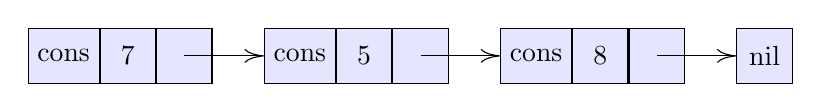
\begin{tikzpicture}
        \matrix (node1) [node_matrix, anchor = west] at (0, 0) {
            \coqinlinelight{cons} &
            7 &
            \\
        };
        \matrix (node2) [node_matrix, anchor = west] at (3, 0) {
            \coqinlinelight{cons} &
            5 &
            \\
        };
        \matrix (node3) [node_matrix, anchor = west] at (6, 0) {
            \coqinlinelight{cons} &
            8 &
            \\
        };
        \matrix (node4) [node_matrix, anchor = west] at (9, 0) {
            \coqinlinelight{nil} \\
        };
        \draw [arrow] (node1-1-3.center) to (node2-1-1);
        \draw [arrow] (node2-1-3.center) to (node3-1-1);
        \draw [arrow] (node3-1-3.center) to (node4-1-1);
    \end{tikzpicture}
\end{center}

\begin{center}
    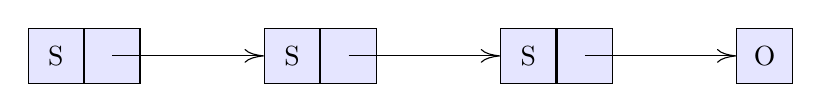
\begin{tikzpicture}
        \matrix (node1) [node_matrix, anchor = west] at (0, 0) {
            \coqinlinelight{S} &
            \\
        };
        \matrix (node2) [node_matrix, anchor = west] at (3, 0) {
            \coqinlinelight{S} &
            \\
        };
        \matrix (node3) [node_matrix, anchor = west] at (6, 0) {
            \coqinlinelight{S} &
            \\
        };
        \matrix (node4) [node_matrix, anchor = west] at (9, 0) {
            \coqinlinelight{O} \\
        };
        \draw [arrow] (node1-1-2.center) to (node2-1-1);
        \draw [arrow] (node2-1-2.center) to (node3-1-1);
        \draw [arrow] (node3-1-2.center) to (node4-1-1);
    \end{tikzpicture}
\end{center}

In fact, we can go from a list to the corresponding natural number by getting its length, and back from a natural number to one of the corresponding lists by repeating an element that many times:

\begin{no_padding_center}
    \begin{tabular}{c c}
        \begin{coq}
Fixpoint length {A} (l : list A) : nat :=
  match l with
  | nil => O
  | cons _ l' => S (length l')
  end.
        \end{coq} &
        \begin{coq}
Fixpoint repeat {A} (x : A) (n : nat) : list A :=
  match n with
  | O => nil
  | S n' => cons x (repeat x n')
  end.
        \end{coq}
    \end{tabular}
\end{no_padding_center}

\section{Binary non-dependent version}

As there are many ways to represent natural numbers (and not only the unary system that was considered above). Depending on which representation we chose, operations on the numbers (such as increment, decrement, sum, converting into other representations) will have different efficiency, and in each case we can find an analogous data structure.

So another simple representation of natural numbers is the binary numeral system. As seen, again, by Chris Okasaki \cite{okasaki_1998}, we can augment it to contain pieces of data by storing a complete binary leaf trees (or nothing) in each digit of the number (although here we will use big-endian digit ordering instead of little-endian).

For the following, we will denote by \coqinline{A} some data type (in examples it will be \coqinline{nat}). A ``complete binary leaf tree'' of depth $d$ has $2^d$ leaves where it stores values of type \coqinline{A} (``complete binary'' meaning that each internal node has exactly 2 children, ``leaf'' meaning that data is only stored in the leaves).

\begin{coq}
Inductive binary_leaf_tree {A} :=
  | BinaryLeafTreeLeaf : A -> binary_leaf_tree
  | BinaryLeafTreeInternalNode : binary_leaf_tree -> binary_leaf_tree -> binary_leaf_tree.

Arguments binary_leaf_tree : clear implicits.
\end{coq}

Here is an example of a complete binary leaf tree of depth $2$ holding values $0$, $1$, $2$, $3$:

\begin{center}
    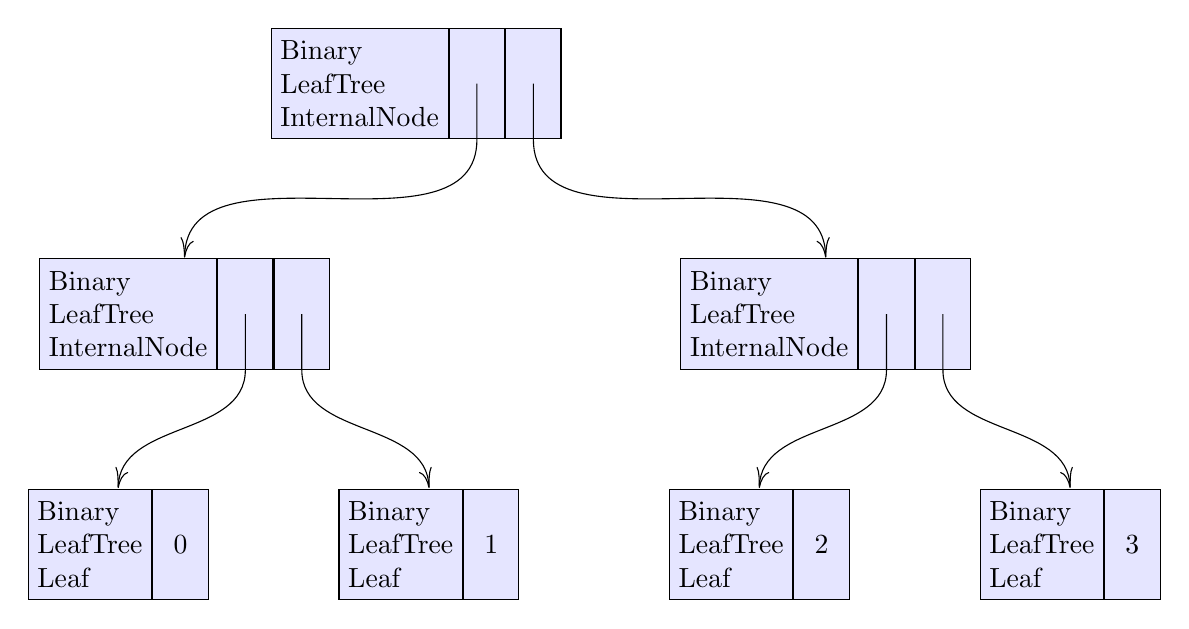
\begin{tikzpicture}
        \matrix (node1) [node_matrix, nodes = {minimum height = 40}, anchor = center] {
            \node (node1-1-1) [align = left] {\coqinlinelight{Binary} \\ \coqinlinelight{LeafTree} \\ \coqinlinelight{InternalNode}}; &
            &
            \\
        };
        \matrix (node2) [node_matrix, nodes = {minimum height = 40}, anchor = center, node distance = 1.5 and 1.5, below left = of node1-1-2] {
            \node (node2-1-1) [align = left] {\coqinlinelight{Binary} \\ \coqinlinelight{LeafTree} \\ \coqinlinelight{InternalNode}}; &
            &
            \\
        };
        \matrix (node3) [node_matrix, nodes = {minimum height = 40}, anchor = center, node distance = 1.5 and 1.5, below right = of node1-1-3] {
            \node (node3-1-1) [align = left] {\coqinlinelight{Binary} \\ \coqinlinelight{LeafTree} \\ \coqinlinelight{InternalNode}}; &
            &
            \\
        };
        \matrix (node4) [node_matrix, nodes = {minimum height = 40}, anchor = center, node distance = 1.5 and 0.1, below left = of node2-1-2] {
            \node (node4-1-1) [align = left] {\coqinlinelight{Binary} \\ \coqinlinelight{LeafTree} \\ \coqinlinelight{Leaf}}; &
            $0$ \\
        };
        \matrix (node5) [node_matrix, nodes = {minimum height = 40}, anchor = center, node distance = 1.5 and 0.1, below right = of node2-1-3] {
            \node (node5-1-1) [align = left] {\coqinlinelight{Binary} \\ \coqinlinelight{LeafTree} \\ \coqinlinelight{Leaf}}; &
            $1$ \\
        };
        \matrix (node6) [node_matrix, nodes = {minimum height = 40}, anchor = center, node distance = 1.5 and 0.1, below left = of node3-1-2] {
            \node (node6-1-1) [align = left] {\coqinlinelight{Binary} \\ \coqinlinelight{LeafTree} \\ \coqinlinelight{Leaf}}; &
            $2$ \\
        };
        \matrix (node7) [node_matrix, nodes = {minimum height = 40}, anchor = center, node distance = 1.5 and 0.1, below right = of node3-1-3] {
            \node (node7-1-1) [align = left] {\coqinlinelight{Binary} \\ \coqinlinelight{LeafTree} \\ \coqinlinelight{Leaf}}; &
            $3$ \\
        };
        \draw [arrow] (node1-1-2.center) -- (node1-1-2.south) to[out = -90, in = 90] (node2.north);
        \draw [arrow] (node1-1-3.center) -- (node1-1-3.south) to[out = -90, in = 90] (node3.north);
        \draw [arrow] (node2-1-2.center) -- (node2-1-2.south) to[out = -90, in = 90] (node4.north);
        \draw [arrow] (node2-1-3.center) -- (node2-1-3.south) to[out = -90, in = 90] (node5.north);
        \draw [arrow] (node3-1-2.center) -- (node3-1-2.south) to[out = -90, in = 90] (node6.north);
        \draw [arrow] (node3-1-3.center) -- (node3-1-3.south) to[out = -90, in = 90] (node7.north);
    \end{tikzpicture}
\end{center}

They will be drawn like that in the future:

\begin{center}
    \completebinaryleaftreedepthtwo{$0$}{$1$}{$2$}{$3$}
\end{center}

We know that for each natural number $n$ there are $d \in \mathbb{N}$ and $n_{d - 1}, n_{d - 2}, ..., n_1, n_0 \in \{0, 1\}$ such that $n = n_{d - 1} 2^{d - 1} + n_{d - 2} 2^{d - 2} + ... + n_1 2^1 + n_0 2^0$. The function \coqinline{to_digits : forall (d n : nat), list nat} gives the list of length \coqinline{d} consisting of these binary digits of \coqinline{n} in big-endian ordering: for example, \coqinline{to_digits 8 73 ~> [0; 1; 0; 0; 1; 0; 0; 1]} (where ``\nospaceevaluatesto'' means ``evaluates to''). The inverse operation is \coqinline{of_digits : forall (d : nat) (nl : list nat), nat}: for example, \coqinline{of_digits 8 [0; 1; 0; 0; 1; 0; 0; 1] ~> 73}.

A ``digital list'' of depth $d$ is a list of length $d$ of which the $k$'th element is a complete binary leaf tree of depth $k$ if $n_k = 1$ and nothing otherwise.

\begin{coq}
Inductive digital_list {A} :=
  | DigitalListNil : digital_list
  | DigitalListCons : option (binary_leaf_tree A) -> digital_list -> digital_list.

Arguments digital_list : clear implicits.
\end{coq}

Here is an example of a digit list for $n = 5$, so we can chose $d = 3$ (the minimum number of bits needed to represent $5$), $n_2$ = 1, $n_1 = 0$, $n_0 = 1$, which stores values 0, 1, 2, 3, 4:

\begin{center}
    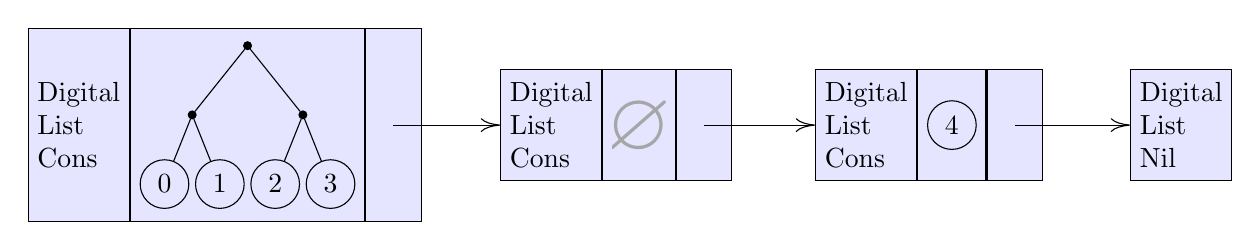
\begin{tikzpicture}
        \matrix (node1) [node_matrix, nodes = {minimum height = 70}, anchor = west] at (0, 0) {
            \node (node1-1-1) [align = left] {\coqinlinelight{Digital} \\ \coqinlinelight{List} \\ \coqinlinelight{Cons}}; &
            \completebinaryleaftreedepthtwo{$0$}{$1$}{$2$}{$3$} &
            \\
        };
        \matrix (node2) [node_matrix, nodes = {minimum height = 40}, anchor = west] at (6, 0) {
            \node (node2-1-1) [align = left] {\coqinlinelight{Digital} \\ \coqinlinelight{List} \\ \coqinlinelight{Cons}}; &
            \bigvarnothing &
            \\
        };
        \matrix (node3) [node_matrix, nodes = {minimum height = 40}, anchor = west] at (10, 0) {
            \node (node3-1-1) [align = left] {\coqinlinelight{Digital} \\ \coqinlinelight{List} \\ \coqinlinelight{Cons}}; &
            \completebinaryleaftreedepthzero{$4$} &
            \\
        };
        \matrix (node4) [node_matrix, nodes = {minimum height = 40}, anchor = west] at (14, 0) {
            \node (node4-1-1) [align = left] {\coqinlinelight{Digital} \\ \coqinlinelight{List} \\ \coqinlinelight{Nil}}; \\
        };
        \draw [arrow] (node1-1-3.center) to (node2-1-1);
        \draw [arrow] (node2-1-3.center) to (node3-1-1);
        \draw [arrow] (node3-1-3.center) to (node4-1-1);
    \end{tikzpicture}
\end{center}

Or, to simplify the drawing, the following notation will be used from now on:

\begin{center}
    $\xbraces{
        \vcenter{\hbox{\completebinaryleaftreedepthtwo{$0$}{$1$}{$2$}{$3$}}};
        \vcenter{\hbox{\bigvarnothing}};
        \vcenter{\hbox{\completebinaryleaftreedepthzero{$4$}}}
    }$
\end{center}

A ``concrete digital list'' is a $d \in \mathbb{N}$ and a digital list of depth $d$ (one of the reasons to store the depth explicitly is so that it can be accessed immediately).

\begin{coq}
Inductive concrete_digital_list {A} :=
  | ConcreteDigitalList : forall (d : nat), digital_list A -> concrete_digital_list.

Arguments concrete_digital_list : clear implicits.
\end{coq}

The following concrete digital list corresponds to the digital list given above:

\begin{center}
    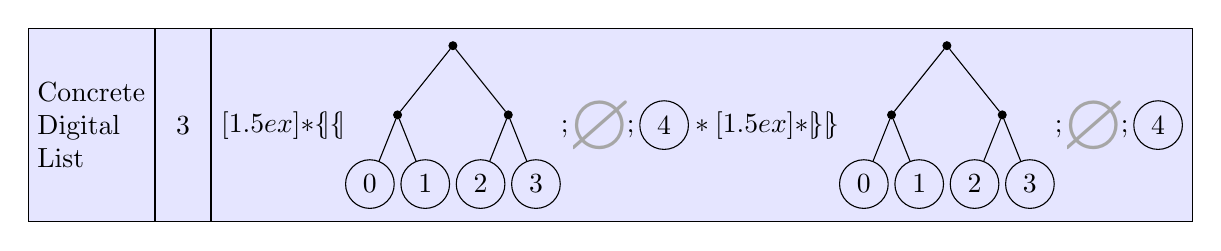
\begin{tikzpicture}
        \matrix (node1) [node_matrix, nodes = {minimum height = 70}, anchor = west] at (0, 0) {
            \node (node1-1-1) [align = left] {\coqinlinelight{Concrete} \\ \coqinlinelight{Digital} \\ \coqinlinelight{List}}; &
            $3$ &
            $\xbraces{
                \vcenter{\hbox{\completebinaryleaftreedepthtwo{$0$}{$1$}{$2$}{$3$}}};
                \vcenter{\hbox{\bigvarnothing}};
                \vcenter{\hbox{\completebinaryleaftreedepthzero{$4$}}}
            }$ \\
        };
    \end{tikzpicture}
\end{center}

Next, we will consider operations that we can do with these types. We will first define each operation on binary leaf trees, then lift it to digital lists (always having a ``depth'' argument, which corresponds to the depth of the digital list passed, for consistency and for reasons outlined later, even when it is not actually used), and finally to concrete digital lists.

\subsection{Interpretation}

The first operation will be conversion to a simple list, which at the same time gives an ``interpretation'' of the data structures, allowing us to establish a connection between the operations on them and ones on the regular lists, which means proving the correctness of these operations.

To convert a binary leaf tree to a list, we just traverse its leaves in their natural order. For example:

\begin{center}
    \coqinline{binary_leaf_tree_to_list}
    $\vcenter{\hbox{\completebinaryleaftreedepthtwo{$0$}{$1$}{$2$}{$3$}}}$
    \coqinline{~> [0; 1; 2; 3]}
\end{center}

\begin{coq}
Fixpoint binary_leaf_tree_to_list {A} (blt : binary_leaf_tree A) :=
  match blt with
  | BinaryLeafTreeLeaf x => [x]
  | BinaryLeafTreeInternalNode blt'1 blt'2 =>
    binary_leaf_tree_to_list blt'1 ++ binary_leaf_tree_to_list blt'2
  end.
\end{coq}

For a digital list, we convert each binary leaf tree (if it exists) to a list and then concatenate the results. For example:

\begin{center}
    \coqinline{digital_list_to_list 3}
    $\xbraces{
        \vcenter{\hbox{\completebinaryleaftreedepthtwo{$0$}{$1$}{$2$}{$3$}}};
        \vcenter{\hbox{\bigvarnothing}};
        \vcenter{\hbox{\completebinaryleaftreedepthzero{$4$}}}
    }$
    \coqinline{~> [0; 1; 2; 3; 4]}
\end{center}

\begin{coq}
Fixpoint digital_list_to_list {A} d (dl : digital_list A) :=
  match dl with
  | DigitalListNil => []
  | DigitalListCons o dl' =>
    match o with
    | None => []
    | Some blt => binary_leaf_tree_to_list blt
    end ++ digital_list_to_list (pred d) dl'
  end.
\end{coq}

The version for concrete digital lists is straight-forward:

\begin{coq}
Definition concrete_digital_list_to_list {A} (cdl : concrete_digital_list A) :=
  let '(ConcreteDigitalList d dl) := cdl in digital_list_to_list d dl.
\end{coq}

\subsection{Creating an empty instance}

Here we just create an empty digital list.

\begin{coq}
Definition digital_list_empty {A} : digital_list A := DigitalListNil.

Definition concrete_digital_list_empty {A} : concrete_digital_list A :=
  ConcreteDigitalList 0 digital_list_empty.
\end{coq}

\subsection{Length}

The length (the number of data elements stored) of a complete binary leaf tree of depth $d$ is, as remarked earlier, $2^d$. So to get the length of a digital list, we just sum the lengths of the binary leaf trees, at positions where they are present. For example:

\begin{center}
    \coqinline{digital_list_length 3}
    $\xbraces{
        \vcenter{\hbox{\completebinaryleaftreedepthtwo{$0$}{$1$}{$2$}{$3$}}};
        \vcenter{\hbox{\bigvarnothing}};
        \vcenter{\hbox{\completebinaryleaftreedepthzero{$4$}}}
    }$
    \coqinline{~> 5}
\end{center}

\begin{coq}
Fixpoint digital_list_length {A} d (dl : digital_list A) :=
  match dl with
  | DigitalListNil => 0
  | DigitalListCons o dl' => (if o then Nat.pow 2 (pred d) else 0) + digital_list_length (pred d) dl'
  end.

Definition concrete_digital_list_length {A} (cdl : concrete_digital_list A) :=
  let '(ConcreteDigitalList d dl) := cdl in digital_list_length d dl.
\end{coq}

\subsection{Getting an element by its index}

The operation of getting the \coqinline{i}th element is a bit more involved. In all cases, we first convert \coqinline{i} to the list of its binary digits, called \coqinline{il} (it has the same length as the depth of the data structure we work with).

Then all we need to do for a complete binary leaf tree is to descend it, starting from the root, taking the left branch if the digit in the current position is $0$ and the right one if the digit in the current position is $1$. For example, suppose we want to get the $6$'th element of the following tree; for that we first convert it to digits (\coqinline{to_digits 3 6 ~> [1; 1; 0]}, where $3$ is the depth of the tree), and then visit the tree as described (the path is highlighted in red):

\begin{center}
    \coqinline{complete_binary_leaf_tree_nth 3 [1; 1; 0]}
    $\vcenter{\hbox{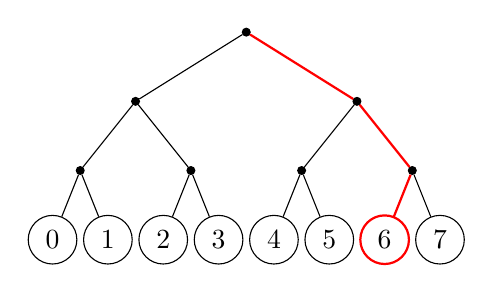
\begin{tikzpicture}
        \begin{scope} [leaf_tree_3]
            \node [style = {leaf_tree_inner_node}] {}
                child {
                    node [style = {leaf_tree_inner_node}] {}
                    child {
                        node [style = {leaf_tree_inner_node}] {}
                        child {
                            node [style = {leaf_tree_leaf}] {0}
                        }
                        child {
                            node [style = {leaf_tree_leaf}] {1}
                        }
                    }
                    child {
                        node [style = {leaf_tree_inner_node}] {}
                        child {
                            node [style = {leaf_tree_leaf}] {2}
                        }
                        child {
                            node [style = {leaf_tree_leaf}] {3}
                        }
                    }
                }
                child {
                    node [style = {leaf_tree_inner_node}] {}
                    child[black, thin] {
                        node [style = {leaf_tree_inner_node}] {}
                        child {
                            node [style = {leaf_tree_leaf}] {4}
                        }
                        child {
                            node [style = {leaf_tree_leaf}] {5}
                        }
                    }
                    child {
                        node[black, thin] [style = {leaf_tree_inner_node}] {}
                        child {
                            node [style = {leaf_tree_leaf}] {6}
                        }
                        child[black, thin] {
                            node [style = {leaf_tree_leaf}] {7}
                        }
                        edge from parent[red, thick]
                    }
                    edge from parent[red, thick]
                };
        \end{scope}
    \end{tikzpicture}}}$
    \coqinline{~> 6}
\end{center}

In this case we suppose that all arguments are valid, but we still have to return an option, as we need to return something in all cases.

\begin{coq}
Fixpoint complete_binary_leaf_tree_nth {A} d il (blt : binary_leaf_tree A) : option A :=
  match il, blt with
  | [], BinaryLeafTreeLeaf x => Some x
  | 0 :: il', BinaryLeafTreeInternalNode blt'1 _ => complete_binary_leaf_tree_nth (pred d) il' blt'1
  | 1 :: il', BinaryLeafTreeInternalNode _ blt'2 => complete_binary_leaf_tree_nth (pred d) il' blt'2
  | _, _ => None
  end.
\end{coq}

Now, consider the following digital list:

\begin{center}
    $\xbraces{
        \vcenter{\hbox{\completebinaryleaftreedepththree{$0$}{$1$}{$2$}{$3$}{$4$}{$5$}{$6$}{$7$}}};
        \vcenter{\hbox{\bigvarnothing}};
        \vcenter{\hbox{\completebinaryleaftreedepthone{$8$}{$9$}}};
        \vcenter{\hbox{\completebinaryleaftreedepthzero{$10$}}}
    }$
\end{center}

To see how to extract the \coqinline{i}th element, we need to know in which it is stored at which index. Let us see on this example what we get:

\begin{center}
    \begin{tabular}{|c|c|c|}
        \hline
        \textbf{Element index} & \textbf{Tree index} & \textbf{Index in tree} \\
        \hline
        $\textcolor{red}{0}000_2$ & $\textcolor{red}{0}$ & $000_2$ \\
        $\textcolor{red}{0}001_2$ & $\textcolor{red}{0}$ & $001_2$ \\
        $\textcolor{red}{0}010_2$ & $\textcolor{red}{0}$ & $010_2$ \\
        $\textcolor{red}{0}011_2$ & $\textcolor{red}{0}$ & $011_2$ \\
        $\textcolor{red}{0}100_2$ & $\textcolor{red}{0}$ & $100_2$ \\
        $\textcolor{red}{0}101_2$ & $\textcolor{red}{0}$ & $101_2$ \\
        $\textcolor{red}{0}110_2$ & $\textcolor{red}{0}$ & $110_2$ \\
        $\textcolor{red}{0}111_2$ & $\textcolor{red}{0}$ & $111_2$ \\
        $10\textcolor{teal}{0}0_2$ & $\textcolor{teal}{2}$ & $0_2$ \\
        $10\textcolor{teal}{0}1_2$ & $\textcolor{teal}{2}$ & $1_2$ \\
        $101\textcolor{blue}{0}_2$ & $\textcolor{blue}{3}$ & $\varepsilon_2$ \\
        \hline
        $\textcolor{red}{1}0\textcolor{teal}{1}\textcolor{blue}{1}_2$ & \multicolumn{2}{|c|}{$\leftarrow$ \textbf{Count of elements in whole digital list}} \\
        \hline
    \end{tabular}
\end{center}

The crucial observation here is that the tree index is the index of the first digit in \coqinline{i} that is strictly less than the corresponding digit of \coqinline{n}, and the index in the tree is just the rest of digits of \coqinline{i}.

So in the case $i_{d - 1} = n_{d - 1} = 0$ (that is, \coqinline{il} starts with 0 and there is no tree in this position) and in the case $i_{d - 1} = n_{d - 1} = 1$ (that is, \coqinline{il} starts with 1 and there is a tree in this position), we recurse to our tail. Otherwise, in the case $i_{d - 1} = 0$ and $n_{d - 1} = 1$ (that is, \coqinline{il} starts with 0 and there is a tree in this position), we ask this tree for its element at position defined by \coqinline{il'}. The case $i_{d - 1} = 1$ and $n_{d - 1} = 0$ is impossible on valid input. \pagebreak% bad

\begin{coq}
Fixpoint digital_list_nth_inner {A} d il (dl : digital_list A) : option A :=
  match il, dl with
  | 0 :: il', DigitalListCons None dl'
  | 1 :: il', DigitalListCons (Some _) dl' => digital_list_nth_inner (pred d) il' dl'
  | 0 :: il', DigitalListCons (Some blt) dl' => complete_binary_leaf_tree_nth (pred d) il' blt
  | _, _ => None
  end.
\end{coq}

All that is left now is to check whether \coqinline{i} is in bounds (to get a function that works forall all \coqinline{i : nat}) and to convert it into digits.

\begin{coq}
Definition digital_list_nth {A} d i (dl : digital_list A) : option A :=
  if Nat.ltb i (digital_list_length d dl)
  then digital_list_nth_inner d (to_digits d i) dl
  else None.

Definition concrete_digital_list_nth {A} i (cdl : concrete_digital_list A) : option A :=
  let '(ConcreteDigitalList d dl) := cdl in digital_list_nth d i dl.
\end{coq}

\subsection{Updating an element by its index}

The operation of replacing the \coqinline{i}th element by another \coqinline{x : A} is completely analogous to getting the \coqinline{i}th element, the only difference is that we reconstruct back the data structures with the element updated.

\begin{coq}
Fixpoint complete_binary_leaf_tree_update {A} d il x (blt : binary_leaf_tree A) :
  option (binary_leaf_tree A) :=
  match il, blt with
  | [], _ => Some (BinaryLeafTreeLeaf x)
  | 0 :: il', BinaryLeafTreeInternalNode blt'1 blt'2 =>
    option_map
      (fun blt'1_0 => BinaryLeafTreeInternalNode blt'1_0 blt'2)
      (complete_binary_leaf_tree_update (pred d) il' x blt'1)
  | 1 :: il', BinaryLeafTreeInternalNode blt'1 blt'2 =>
    option_map
      (fun blt'2_0 => BinaryLeafTreeInternalNode blt'1 blt'2_0)
      (complete_binary_leaf_tree_update (pred d) il' x blt'2)
  | _, _ => None
  end.

Fixpoint digital_list_update_inner {A} d il x (dl : digital_list A) : option (digital_list A) :=
  match il, dl with
  | 0 :: il', DigitalListCons (None as o) dl'
  | 1 :: il', DigitalListCons (Some _ as o) dl' =>
    option_map
      (DigitalListCons o)
      (digital_list_update_inner (pred d) il' x dl')
  | 0 :: il', DigitalListCons (Some blt) dl' =>
    Some (DigitalListCons (complete_binary_leaf_tree_update (pred d) il' x blt) dl')
  | _, _ => None
  end.

Definition digital_list_update {A} d i x (dl : digital_list A) : option (digital_list A) :=
  if Nat.ltb i (digital_list_length d dl)
  then digital_list_update_inner d (to_digits d i) x dl
  else None.

Definition concrete_digital_list_update {A} i x (cdl : concrete_digital_list A) :
  option (concrete_digital_list A) :=
  let '(ConcreteDigitalList d dl) := cdl in
    option_map (ConcreteDigitalList d) (digital_list_update d i x dl).
\end{coq}

\subsection{Adding an element to the end}

Adding an element \coqinline{x : A} to the end of a digital list of depth \coqinline{d} can potentially produce a carry (a complete binary leaf tree of depth \coqinline{d}) and always gives a digital list of the same depth \coqinline{d}.

If the initial digital list is of depth $0$, we output a carry with the element \coqinline{x}. For example:

\begin{center}
    \coqinline{digital_list_push 0 8}
    $\xbraces{
        \vcenter{\hbox{\spacer}}
    }$
    \evaluatesto
    $\left(
        \,\vcenter{\hbox{\completebinaryleaftreedepthzero{$8$}}}\,,
        \xbraces{
            \vcenter{\hbox{\spacer}}
        }
    \right)$
\end{center}

Else, we recurse. Suppose that we did not get a carry. In this case, we just add our digit (if it exists) to the result of the recursive call. For example, if the recursive call looked like this:

\begin{center}
    \coqinline{digital_list_push 2 8}
    $\xbraces{
        \vcenter{\hbox{\completebinaryleaftreedepthone{$4$}{$5$}}};
        \vcenter{\hbox{\bigvarnothing}}
    }$
    \evaluatesto
    $\left(
        \vcenter{\hbox{\bigvarnothing}}\,,
        \xbraces{
            \vcenter{\hbox{\completebinaryleaftreedepthone{$4$}{$5$}}};
            \vcenter{\hbox{\completebinaryleaftreedepthzero{$8$}}}
        }
    \right)$
\end{center}

Then the parent execution can be the following:

\begin{center}
    \coqinline{digital_list_push 3 8}
    $\xbraces{
        \vcenter{\hbox{\completebinaryleaftreedepthtwo{$0$}{$1$}{$2$}{$3$}}};
        \vcenter{\hbox{\completebinaryleaftreedepthone{$4$}{$5$}}};
        \vcenter{\hbox{\bigvarnothing}}
    }$
    \evaluatesto
    $\left(
        \vcenter{\hbox{\bigvarnothing}}\,,
        \xbraces{
            \vcenter{\hbox{\completebinaryleaftreedepthtwo{$0$}{$1$}{$2$}{$3$}}};
            \vcenter{\hbox{\completebinaryleaftreedepthone{$4$}{$5$}}};
            \vcenter{\hbox{\completebinaryleaftreedepthzero{$8$}}}
        }
    \right)$
\end{center}

Else there was a carry. And again, the are two cases, depending on whether or not the head of the digital list contains a tree. If it does not, we just add the carry that we got in this place. For example, if the recursive call looked like this:

\begin{center}
    \coqinline{digital_list_push 2 8}
    $\xbraces{
        \vcenter{\hbox{\completebinaryleaftreedepthone{$0$}{$1$}}};
        \vcenter{\hbox{\completebinaryleaftreedepthzero{$2$}}}
    }$
    \evaluatesto
    $\left(
        \,\vcenter{\hbox{\completebinaryleaftreedepthtwo{$0$}{$1$}{$2$}{$8$}}}\,,
        \xbraces{
            \vcenter{\hbox{\bigvarnothing}};
            \vcenter{\hbox{\bigvarnothing}}
        }
    \right)$
\end{center}

Then the parent execution can be the following:

\begin{center}
    \coqinline{digital_list_push 3 8}
    $\xbraces{
        \vcenter{\hbox{\bigvarnothing}};
        \vcenter{\hbox{\completebinaryleaftreedepthone{$0$}{$1$}}};
        \vcenter{\hbox{\completebinaryleaftreedepthzero{$2$}}}
    }$
    \evaluatesto
    $\left(
        \vcenter{\hbox{\bigvarnothing}}\,,
        \xbraces{
            \vcenter{\hbox{\completebinaryleaftreedepthtwo{$0$}{$1$}{$2$}{$8$}}};
            \vcenter{\hbox{\bigvarnothing}};
            \vcenter{\hbox{\bigvarnothing}}
        }
    \right)$
\end{center}

But if the head of the list contains a tree, then we create a tree from it and the carry and return it again as a carry. For example, if the recursive call looked like this:

\begin{center}
    \coqinline{digital_list_push 1 8}
    $\xbraces{
        \vcenter{\hbox{\completebinaryleaftreedepthzero{$2$}}}
    }$
    \evaluatesto
    $\left(
        \,\vcenter{\hbox{\completebinaryleaftreedepthone{$2$}{$8$}}}\,,
        \xbraces{
            \vcenter{\hbox{\bigvarnothing}}
        }
    \right)$
\end{center}

Then the parent execution can be the following:

\begin{center}
    \coqinline{digital_list_push 2 8}
    $\xbraces{
        \vcenter{\hbox{\completebinaryleaftreedepthone{$0$}{$1$}}};
        \vcenter{\hbox{\completebinaryleaftreedepthzero{$2$}}}
    }$
    \evaluatesto
    $\left(
        \,\vcenter{\hbox{\completebinaryleaftreedepthtwo{$0$}{$1$}{$2$}{$8$}}}\,,
        \xbraces{
            \vcenter{\hbox{\bigvarnothing}};
            \vcenter{\hbox{\bigvarnothing}}
        }
    \right)$
\end{center}

We can remark an analogy with binary adders:

\begin{center}
    \newcolumntype{M}{>{\centering\arraybackslash}m{45pt}}

    \begin{tabular}{|M|M||M|M|}
        \hline
        \textbf{First operand} & \textbf{Second operand} & \textbf{Carry} & \textbf{Result} \\
        \hline
        $0$ & $0$ & $0$ & $0$ \\
        $0$ & $1$ & $0$ & $1$ \\
        $1$ & $0$ & $0$ & $1$ \\
        $1$ & $1$ & $1$ & $0$ \\
        \hline
    \end{tabular}
\end{center}

\begin{coq}
Fixpoint digital_list_push {A} d x (dl : digital_list A) : option (binary_leaf_tree A) * (digital_list A) :=
  match dl with
  | DigitalListNil => (Some (BinaryLeafTreeLeaf x), DigitalListNil)
  | DigitalListCons o dl' =>
    match digital_list_push (pred d) x dl' with
    | (None, dl'0) => (None, DigitalListCons o dl'0)
    | (Some blt0, dl'0) =>
      match o with
      | None => (None, DigitalListCons (Some blt0) dl'0)
      | Some blt => (Some (BinaryLeafTreeInternalNode blt blt0), DigitalListCons None dl'0)
      end
    end
  end.
\end{coq}

To get a concrete digital list from an optional carry and the resulting digital list, we add the carry to the head of the digital list if it exists (and get a digital list of depth one more than the original), if not, then just return the digital list from the operation.

\begin{coq}
Definition concrete_digital_list_push {A} x (cdl : concrete_digital_list A) : concrete_digital_list A :=
  let '(ConcreteDigitalList d dl) := cdl in
    match digital_list_push d x dl with
    | (None, dl0) => ConcreteDigitalList d dl0
    | (Some blt0, dl0) => ConcreteDigitalList (S d) (DigitalListCons (Some blt0) dl0)
    end.
\end{coq}

\subsection{Removing an element from the end}

To remove the last element from a complete binary leaf tree, we split it into a digital list and this element. For example:

\begin{center}
    \coqinline{complete_binary_leaf_tree_pop}
    $\vcenter{\hbox{\completebinaryleaftreedepththree{$0$}{$1$}{$2$}{$3$}{$4$}{$5$}{$6$}{$7$}}}$
    \evaluatesto
    $\left(
        \xbraces{
            \vcenter{\hbox{\completebinaryleaftreedepthtwo{$0$}{$1$}{$2$}{$3$}}};
            \vcenter{\hbox{\completebinaryleaftreedepthone{$4$}{$5$}}};
            \vcenter{\hbox{\completebinaryleaftreedepthzero{$6$}}}
        },
        7
    \right)$
\end{center}

\begin{coq}
Fixpoint complete_binary_leaf_tree_pop {A} d (blt : binary_leaf_tree A) : digital_list A * A :=
  match blt with
  | BinaryLeafTreeLeaf x => (DigitalListNil, x)
  | BinaryLeafTreeInternalNode blt'1 blt'2 =>
    let '(dl', x) := complete_binary_leaf_tree_pop (pred d) blt'2 in
      (DigitalListCons (Some blt'1) dl', x)
  end.
\end{coq}

To remove the last element of a digital list, we just recurse until we are at the last existing tree, from which we remove the element from the end, and then reconstruct back the digital list, leaving unchanged all of the previous trees. For example:

\begin{center}
    \coqinline{digital_list_pop 3 8}
    $\xbraces{
        \vcenter{\hbox{\completebinaryleaftreedepthtwo{$0$}{$1$}{$2$}{$3$}}};
        \vcenter{\hbox{\completebinaryleaftreedepthone{$4$}{$5$}}};
        \vcenter{\hbox{\bigvarnothing}}
    }$
    \evaluatesto
    $\left(
        \xbraces{
            \vcenter{\hbox{\completebinaryleaftreedepthtwo{$0$}{$1$}{$2$}{$3$}}};
            \vcenter{\hbox{\bigvarnothing}};
            \vcenter{\hbox{\completebinaryleaftreedepthzero{$4$}}}
        },
        5
    \right)$
\end{center}

The only case when we return $\varnothing$ is when the original digital list does not contain trees. For example:

\begin{center}
    \coqinline{digital_list_pop 2 8}
    $\xbraces{
        \vcenter{\hbox{\bigvarnothing}};
        \vcenter{\hbox{\bigvarnothing}}
    }$
    \evaluatesto
    $\vcenter{\hbox{\bigvarnothing}}$
\end{center}

We do not try to maintain the minimum possible depth, so the head of the digital list can become empty. \pagebreak% bad

\begin{coq}
Fixpoint digital_list_pop {A} d (dl : digital_list A) : option (digital_list A * A) :=
  match dl with
  | DigitalListNil => None
  | DigitalListCons o dl' =>
    match digital_list_pop (pred d) dl' with
    | None =>
      option_map
        (fun blt =>
          let '(dl'0, x) := complete_binary_leaf_tree_pop (pred d) blt in
            (DigitalListCons None dl'0, x)
        )
        o
    | Some (dl'0, x) => Some (DigitalListCons o dl'0, x)
    end
  end.

Definition concrete_digital_list_pop {A} (cdl : concrete_digital_list A) :
  option (concrete_digital_list A * A) :=
  let '(ConcreteDigitalList d dl) := cdl in
    option_map
      (fun '(dl0, x) => (ConcreteDigitalList d dl0, x))
      (digital_list_pop d dl).
\end{coq}

\section{\texttt{r}-ary dependent version}

So far we have only defined functions, but did not proven them correct. But that will be complicated by the fact that our data structures can have invalid values. For example, this is representable and has type \coqinline{concrete_digital_list nat}:

\begin{center}
    \begin{tikzpicture}
        \matrix (node1) [node_matrix, nodes = {minimum height = 70}, anchor = west] at (0, 0) {
            \node (node1-1-1) [align = left] {\coqinlinelight{Concrete} \\ \coqinlinelight{Digital} \\ \coqinlinelight{List}}; &
            $6322$ &
            $\xbraces{
                \vcenter{\hbox{\bigvarnothing}};
                \vcenter{\hbox{\completebinaryleaftreedepthzero{$4$}}};
                \vcenter{\hbox{\begin{tikzpicture}%
                    \begin{scope} [leaf_tree_2]
                        \node [style = {leaf_tree_inner_node}] {}
                            child {
                                node [style = {leaf_tree_inner_node}] {}
                                child {
                                    node [style = {leaf_tree_leaf}] {$0$}
                                }
                                child {
                                    node [style = {leaf_tree_leaf}] {$1$}
                                }
                            }
                            child {
                                node [style = {leaf_tree_leaf}] {$2$}
                            };
                    \end{scope}
                \end{tikzpicture}}}
            }$ \\
        };
    \end{tikzpicture}
\end{center}

To fix that, we could just define predicates that assert that the data structures are valid, and that option was also tried. But here we will explore another way to achieve what we want: dependent types, which allow to store proofs of data structure invariants inside data structures themselves.

One example is a ``sized list'', which is a type of lists that are guaranteed to have the length given in their type.

\begin{coq}
Inductive sized_list {A} : nat -> Type :=
  | SizedListNil : sized_list 0
  | SizedListCons : forall {n}, A -> sized_list n -> sized_list (S n).

Arguments sized_list : clear implicits.

Notation "x :||: l" := (SizedListCons x l) (at level 51, right associativity).

Notation "[| |]" := SizedListNil (format "[| |]").
Notation "[| x |]" := (SizedListCons x SizedListNil).
Notation "[| x ; y ; .. ; z |]" := (SizedListCons x (SizedListCons y .. (SizedListCons z SizedListNil) ..)).
\end{coq}

For example, \coqinline{[|1; 2; 3|] : sized_list nat 3}.

But there is another problem, that of efficiency. Storing binary trees means that a lot of memory is wasted on pointers, which also take time to access. To solve this, we can store not binary trees, but \coqinline{r}-ary trees. We call this \coqinline{r} (a natural number greater than one) the ``radix'' of the data structure. Everything we have seen so far generalizes naturally to any such radix, and not just $2$.

We will use \coqinline{r}-ary complete trees instead of binary complete trees. Also, we will store between $0$ and \coqinline{r - 1} of these trees in each position of a digital tree, and not $0$ or $1$ as before (represented by the \coqinline{option} type).

To store something repeated number of times, we need (functional) arrays. To model them in Coq, we will just create a wrapper around sized lists and define some operations on it that forward to ones on sized lists. But we will assume this knowledge of internal representation only in proofs, and in computational contents we will only use the operations defined directly on arrays.

\begin{coq}
Inductive array {A n} :=
  | Array : sized_list A n -> array.

Arguments array : clear implicits.
\end{coq}

The definition of the type of a complete leaf tree is actually a function that computes the type consisting of nested arrays of given radix and depth.

\begin{coq}
Fixpoint complete_leaf_tree A r d :=
  match d with
  | 0 => A
  | S d' => array (complete_leaf_tree A r d') r
  end.
\end{coq}

For example, \coqinline{complete_leaf_tree nat 2 3 ~> array (array (array nat 2) 2) 2}. And here is an example of a term of this type:

\begin{coq}
Check
    Array [|
        Array [|
            Array [|0; 1|];
            Array [|2; 3|]
        ];
        Array [|
            Array [|4; 5|];
            Array [|6; 7|]
        |]
    |]
    : complete_leaf_tree nat 2 3.
\end{coq}

The definitions of a digital list and a concrete digital list are similar to the ones seen before, but now, as promised, contain requirements that make data structures of these types always valid. Here \coqinline{k} is the number of trees at a position of digital trees, and it, as said before, will be a natural number strictly less than \coqinline{r}.

\begin{coq}
Inductive digital_list {A r} : nat -> Type :=
  | DigitalListNil : digital_list 0
  | DigitalListCons :
      forall {d} k,
      k < r ->
      array (complete_leaf_tree A r d) k ->
      digital_list d ->
      digital_list (S d).

Arguments digital_list : clear implicits.

Inductive concrete_digital_list {A r} :=
  | ConcreteDigitalList : forall d, digital_list A r d -> concrete_digital_list.

Arguments concrete_digital_list : clear implicits.
\end{coq}

Now we define the operations on them. In the end, here is the types of ones on concrete digital lists look like:

\begin{coq}
Check concrete_digital_list_to_list : forall {A} {r}, concrete_digital_list A r -> list A.
Check concrete_digital_list_empty : forall {A} {r}, concrete_digital_list A r.
Check concrete_digital_list_length : forall {A} {r}, concrete_digital_list A r -> nat.
Check concrete_digital_list_nth : forall {A} {r} (i : nat), concrete_digital_list A r -> option A.
Check concrete_digital_list_update : forall {A} {r}, nat -> A -> concrete_digital_list A r ->
  option (concrete_digital_list A r).
Check concrete_digital_list_push : forall {A} {r}, A -> concrete_digital_list A r -> concrete_digital_list A r.
Check concrete_digital_list_pop : forall {A} {r}, concrete_digital_list A r ->
  option (concrete_digital_list A r * A).
\end{coq} \pagebreak% bad

And here is an example of how implementation of an operation can look like:

\begin{coq}
Fixpoint digital_list_nth_inner {A r d} (isl : sized_list nat d) (dl : digital_list A r d)
  {struct dl} : option A :=
  match dl with
  | DigitalListNil => fun (isl : sized_list nat 0) =>
    None
  | @DigitalListCons _ _ d' k _ a dl' => fun (isl : sized_list nat (S d')) =>
    match isl with
    | @SizedListCons _ d'0 i isl'0 => fun (Heqd : S d'0 = S d') =>
      let isl' := rew (eq_add_S _ _ Heqd) in isl'0 in
      if Nat.eqb i k
      then digital_list_nth_inner isl' dl'
      else option_flat_map (complete_leaf_tree_nth isl') (array_nth i a)
    end eq_refl
  end isl.
\end{coq}

As can be seen, some work in necessary to obtain and use all of the equalities needed to analyze cases and to issue recursive calls with correct types. Here we can see why the \coqinline{d} argument is indispensable with dependent types.

Then we show correctness of the operations by proving that they perform the same operations as ones on corresponding regular lists. Here are the theorem statements about concrete digital lists:

\begin{coq}
Theorem concrete_digital_list_empty_correct :
  forall {A r},
  concrete_digital_list_to_list (concrete_digital_list_empty : concrete_digital_list A r) = [].

Theorem concrete_digital_list_length_correct :
  forall {A r} (cdl : concrete_digital_list A r),
  concrete_digital_list_length cdl = length (concrete_digital_list_to_list cdl).

Theorem concrete_digital_list_nth_correct :
  forall {A r} i (cdl : concrete_digital_list A r),
  r > 1 ->
  concrete_digital_list_nth i cdl = List.nth_error (concrete_digital_list_to_list cdl) i.

Theorem concrete_digital_list_update_correct :
  forall {A r} i x (cdl : concrete_digital_list A r),
  r > 1 ->
  option_map concrete_digital_list_to_list (concrete_digital_list_update i x cdl) =
    list_update i x (concrete_digital_list_to_list cdl).

Theorem concrete_digital_list_push_correct :
  forall {A r} x (cdl : concrete_digital_list A r),
  r > 1 ->
  concrete_digital_list_to_list (concrete_digital_list_push x cdl) =
    concrete_digital_list_to_list cdl ++ [x].

Theorem concrete_digital_list_pop_correct :
  forall {A r} (cdl : concrete_digital_list A r),
  r > 1 ->
  option_map
    (fun '(cdl0, x) => (concrete_digital_list_to_list cdl0, x))
    (concrete_digital_list_pop cdl) = list_pop (concrete_digital_list_to_list cdl).
\end{coq}

\section{\texttt{r}-ary non-dependent version}

But we can nonetheless make a non-dependent version to be able to compare it to the dependent one. Here we base arrays on regular lists and not on sized lists.

\begin{coq}
Inductive array {A} :=
  | Array : list A -> array.

Arguments array : clear implicits.
\end{coq}

And here is how we define complete leaf trees, digital lists and concrete digital lists, as well as predicates of their validity:

\begin{coq}
Inductive leaf_tree {A} :=
  | LeafTreeLeaf : A -> leaf_tree
  | LeafTreeInternalNode : array leaf_tree -> leaf_tree.

Arguments leaf_tree : clear implicits.

Inductive leaf_tree_complete {A} r : nat -> leaf_tree A -> Prop :=
  | LeafTreeCompleteLeaf : forall x, leaf_tree_complete r 0 (LeafTreeLeaf x)
  | LeafTreeCompleteInternalNode :
      forall {d} a,
      array_length a = r ->
      List.Forall (leaf_tree_complete r d) (array_to_list a) ->
      leaf_tree_complete r (S d) (LeafTreeInternalNode a).

Inductive digital_list {A} :=
  | DigitalListNil : digital_list
  | DigitalListCons : array (leaf_tree A) -> digital_list -> digital_list.

Arguments digital_list : clear implicits.

Inductive concrete_digital_list {A} :=
  | ConcreteDigitalList : forall (d : nat), digital_list A -> concrete_digital_list.

Arguments concrete_digital_list : clear implicits.

Inductive digital_list_good {A} r : nat -> digital_list A -> Prop :=
  | DigitalListGoodNil : digital_list_good r 0 DigitalListNil
  | DigitalListGoodCons :
      forall {d} (a : array (leaf_tree A)) (dl : digital_list A),
      array_length a < r ->
      List.Forall (leaf_tree_complete r d) (array_to_list a) ->
      digital_list_good r d dl ->
      digital_list_good r (S d) (DigitalListCons a dl).
\end{coq}

And how we have to not only show that the operations do indeed perform the required actions on data structures, but also that they preserve validity, so we prove 2 theorems each time. For example:

\begin{coq}
Theorem concrete_digital_list_push_correct :
  forall {A} r x (cdl : concrete_digital_list A),
  concrete_digital_list_good r cdl ->
  r > 1 ->
  concrete_digital_list_to_list r (concrete_digital_list_push r x cdl) =
    concrete_digital_list_to_list r cdl ++ [x].

Theorem concrete_digital_list_push_good :
  forall {A} r x (cdl : concrete_digital_list A),
  concrete_digital_list_good r cdl ->
  r > 1 ->
  concrete_digital_list_good r (concrete_digital_list_push r x cdl).
\end{coq}

\section{Extraction}

Now we can extract what we got into OCaml, mapping functions used to standard ones where possible. For example, here is how extracted arrays (in the dependent version) are implemented as functional arrays, using the normal array type of OCaml; as an array is never actually constructed or destructed directly, we can write \coqinline{assert false} in these implementations:

\begin{coq}
Extract Inductive array => ``array'' [ ``(assert false)'' ] ``(assert false)''.
Extract Constant array_to_list => ``fun _ a -> Array.to_list a''.
Extract Inlined Constant array_empty => ``[||]''.
Extract Constant array_single => ``fun x -> [|x|]''.
\end{coq}
\pagebreak% bad
\begin{coq}
Extract Constant array_nth => ``
  fun _ i a ->
    try Some a.(i)
    with Invalid_argument _ -> None
''.
Extract Constant array_update => ``
  fun _ i x a ->
    let a0 = Array.copy a in
    try
      a0.(i) <- x;
      Some a0
    with Invalid_argument _ -> None
''.
Extract Constant array_push => ``
  fun n x a ->
    let a0 = Array.make (n + 1) x in
    Array.blit a 0 a0 0 n;
    a0
''.
Extract Constant array_pop => ``fun n a -> (Array.sub a 0 n, a.(n))''.
\end{coq}

For the dependent and the non-dependent version, we get functions of the same types, so we can put them in a module:

\begin{coq}
module type DIGITAL_LIST = sig
  type 'a concrete_digital_list
  val concrete_digital_list_to_list : int -> 'a concrete_digital_list -> 'a list
  val concrete_digital_list_length : int -> 'a concrete_digital_list -> int
  val concrete_digital_list_empty : int -> 'a concrete_digital_list
  val concrete_digital_list_nth : int -> int -> 'a concrete_digital_list -> 'a option
  val concrete_digital_list_update :
    int -> int -> 'a -> 'a concrete_digital_list -> 'a concrete_digital_list option
  val concrete_digital_list_push : int -> 'a -> 'a concrete_digital_list -> 'a concrete_digital_list
  val concrete_digital_list_pop : int -> 'a concrete_digital_list -> ('a concrete_digital_list * 'a) option
end
\end{coq}

Then we can write a test program, that does some operations on each implementation and outputs some statistics on memory usage:

\begin{coq}
let time l =
  let t = Sys.time() in
  let v = Lazy.force l in
  Printf.printf "Execution time: %fs\n" (Sys.time() -. t);
  flush stdout;
  v

let measure_size x = (Marshal.to_bytes x [] |> Bytes.length |> float_of_int) /. 1024.0 /. 1024.0

module Example = functor (Dl : Digital_list.DIGITAL_LIST) -> struct
  open Dl

  let main =
    time (lazy (
      let r = 32 in
      let cdl = concrete_digital_list_empty r |> ref in
      for _ = 0 to 10000000 do
        cdl := !cdl |> concrete_digital_list_push r 0
      done;
      for i = 0 to (!cdl |> concrete_digital_list_length r) - 1 do
        cdl := !cdl |> concrete_digital_list_update r i (i mod 123) |> Option.get
      done;
      let a = Array.make (!cdl |> concrete_digital_list_length r) 0 in
      for i = 0 to (!cdl |> concrete_digital_list_length r) - 1 do
        a.(i) <- !cdl |> concrete_digital_list_nth r i |> Option.get
      done;
      Printf.printf "Raw data size (after serialization): %f MiB\n" (a |> measure_size);
      Printf.printf "Data structure size (after serialization): %f MiB\n" (cdl |> measure_size)
    ))
end

let _ = Printf.printf "Dependent version:\n"

module Example_dep = Example(Digital_list.Dep)

let _ = Printf.printf "Non-dependent version:\n"

module Example_non_dep = Example(Digital_list.Non_dep)
\end{coq}

Here is the output of one particular execution:

\begin{coq}
Dependent version:
Raw data size (after serialization): 14.111297 MiB
Data structure size (after serialization): 15.649498 MiB
Execution time: 8.290652s
Non-dependent version:
Raw data size (after serialization): 14.111297 MiB
Data structure size (after serialization): 25.493868 MiB
Execution time: 11.857548s
\end{coq}

Even though this way of measuring data structure size is very crude, we can still note that the extraction of the dependent version works faster and uses less memory than the non-dependent one. The reason is that the non-dependent version needs more indirections when storing leaf trees, which are bad for performance and for memory footprint.

An interesting remark is that the extraction of the dependent version contains some unsafe casts (\coqinline{Obj.magic}), as otherwise the polymorphic recursion used would be hard or impossible to do in OCaml directly. But that is fine, because we have proven that everything is correct at the time of defining terms (as they type check, by correctness of extraction the end result should not perform any wrong casts). And otherwise, by writing OCaml code directly, we would not have such guarantees, meaning that there can be unexpected bugs or even security vulnerabilities if \coqinline{Obj.magic} was used wrongly.

For the choice of \coqinline{r}, here is how much time executing the code above (but with $1000000$ as digital lists length) for the dependent version takes for different values of \coqinline{r} (logarithmic scale):

\begin{center}
    \begin{tikzpicture}
        \begin{axis}[xlabel = \coqinline{r}, ylabel = {Time (ms, lower is better)}, xlabel shift = -30, ylabel shift = -40, xmode = log, log basis x = 2, width = \textwidth, height = 10cm]
            \addplot[mark = none] table [x = r, y = time, col sep = comma] {../extraction/rs_output.csv};
        \end{axis}
    \end{tikzpicture}
\end{center}

We can see that the optimal radix in this particular case is around $32$. We can also remark that the binary case is many times slower, and so generalizing the data structure to different radixes can actually be useful for some scenarios.

\section{Methodology}

First, the \coqinline{r}-ary dependent version was done, from it the \coqinline{r}-ary non-dependent one was obtained, and finally it was specialized to \coqinline{r = 2} to get the binary non-dependent version.

Using dependent types means that the functions that perform operations have to be decorated with proofs, but that is, in some sense, a good thing: this catches a lot of mistakes (as it limits what it is possible to write, it is harder to construct wrong expressions); it took some time to construct the terms of the functions, but the first time it type checked, it was already correct.

Here are some statics on development sizes:

\begin{center}
    \begin{tabular}{|l|r|}
        \hline
        \href{https://github.com/afdw/digital_list/blob/main/theories/Utils.v}{Common code} & 426 lines of code \\
        \hline
        \href{https://github.com/afdw/digital_list/tree/main/theories/Dep}{\coqinlinelight{r}-ary dependent version} & 1030 lines of code \\
        \hline
        \href{https://github.com/afdw/digital_list/tree/main/theories/NonDep}{\coqinlinelight{r}-ary non-dependent version} & 1107 lines of code \\
        \hline
    \end{tabular}
\end{center}

We can see that the non-dependent version turned out to be longer, but this may be due to the fact that it was adapted from the dependent one and not done directly.

The benefit of the non-dependent version is that the implementations of operations are more readable, because they are not cluttered with proofs.

The source code of the development is available at \url{https://github.com/afdw/digital_list}.

\section{Related work}

There are other developments similar to the one described here exists, notably proofs of binary random access lists \cite{cfml_binary_random_access_lists} and finger trees \cite{cfml_finger_trees} by Arthur Charguéraud. The notable difference is that the implementations are written in OCaml, and then they are extracted and proved in Coq using the CFML framework \cite{cfml}, whereas this development was done in Coq and then extracted in OCaml (so in the opposite direction).

There are other formalizations of data structures using dependent types, for example, again, finger trees in Coq by Matthieu Sozeau \cite{program_ing_finger_trees_in_coq}.

\printbibliography

\end{document}
